\chapter {卷积神经网络的相关技术介绍}
在这一章中主要介绍涉及人脸属性的一些深度学习基本常识如卷积神经网络的基本操作、训练方法等;也会介绍具体的工程实现过程和相关的瓶颈优化如:多机多卡训练的同步训练方式和异步训练方式、网络前馈中对于卷积操作的优化算法,工程中使用向量处理器结合向量指令集完成对于卷积操作的加速等。这些工作都是我整个研究生生涯花费了大量的精力去理解并且思考的,在很多地方也总结了一些看法和规律,在我的研究生科研和工作过程中起到了非常重要的作用。

\section{卷积神经网络的基础操作和训练}
卷积神经网络一般是指是针对以共享式多通道卷积操作为代表的一连串数学操作计算组合的一个总称,因为卷积计算是其中的主要计算过程和核心特征提取方式,而计算的过程往往需要加入一步非线性的激活函数用以增加整个计算过程对于非线性过程的模拟,这个过程和人体的神经元结构非常相似,所以从计算科学的角度称为卷积神经网络。由于卷积神经网络具有参数多,训练数据广的特点,难以通过正常的线性代数和微积分求得最优解,一般会使用反向传播算法\cite{BP}进行训练,也称梯度下降算法。

在图像识别领域中,卷积神经网络和普通的神经网络,玻尔兹曼感知机等很像:
都是把输入数据最后转化成输出;都要使用输入并进行点积运算;
都使用可以学习参数的神经元;神经元都含有非线性激活函数;
在最后都加入分类的损失函数等等。

而卷积神经网络,借鉴于其常见的多维向量点乘的结构的设计,使其对于图像的2d结构具有良好的亲和性,利用这个特点,基于图像的卷积神经网络结构层出不穷,各自的识别效果也几乎是节节攀升。 
接下来,笔者将从基本网络结构的组成、常用非线性激活函数、常用初始化参数方法、卷积神经网络的训练与 优化四个方面来介绍卷积神经网络的相关内容。
\subsection{卷积神经网络结构的基本组成}
层是卷积神经网络结构的基本组成单位,不同的网络结构中都是使用类似或者基础的层来进行搭建完成,少则三、四层,多达成百上千,但无论是深度还是广度的扩增,都是通过增加层的使用来完成。
\subsubsection{卷积层}
卷积层\cite{ALEXNET}是卷积神经网络最重要的层,因为卷积层承担着从图像到高层语义的转化任务,实际使用中也占据了整个网络计算量中的绝大部分。
甚至毫不客气地讲,对于卷积层的实现和优化好坏,决定着一个深度学习框架的工作使命和存在意义。(最直观的例子就是最著名的卷积神经网络框架caffe就是因为对于卷积的实现做得好,训练和测试的速度较快,从而取代了cuda convnet和CXXnet成了主流,也是目前影响最深的深度学习框架。)

具体来讲:每一个卷积层都会使用N个不同参数的卷积滤波器核,每一个卷积滤波器核对整个输入特征图进行卷积操作,在这个卷积过程中是只是用那一个核的参数,也就是所谓的参数共享。 
参数层面:卷积滤波器核超参数包括:
\begin{enumerate}
\item N 卷积滤波器核数目
\item $Kernel_h$,$Kernel_w$ 卷积滤波器核高度和宽度
\item $Stride_h$,$Stride_w$ 卷积在高、宽维上的步长
\item $PadH$,$PadW$ 对于高、宽二维上对于feature map的空白补足
\end{enumerate}
输入输出参数:\begin{enumerate}
\item $Coutput$,$Houtput$,$Woutput$ 分别为输出通道数、输出高度、输出宽度
\item $Cinput$,$Hinput$,$Winput$    分别为输入通道数、输入高度、输入宽度
\end{enumerate}
其中输出参数由如下公式确定:
\begin{equation}{
\begin{split}
 & Woutput= \frac{Winput-KernelW}{StrideW} +1 \\
 & Houtput= \frac{Hinput-KernelH}{StrideH} +1 \\
 & Coutput= N
\end{split}
}\end{equation}

卷积层的内部参数包括权重$W$和偏置 $b$,
\begin{enumerate}
\item $W$是一个维数是$ Coutput*Cinput*KernelH*KernelW $多维数组.
\item $b$是维数为$Coutput*1$的数组。
\end{enumerate}

卷积的基本计算公式如下: 
\begin{equation}{
 x_j=f(\sum_{i\in (convscale) }x_i*W_i+b_j ) 
}
\end{equation}

convscale是指对应一次卷积操作中对应的$Coutput*kernel_h*kernel_w$范围内的输入图片和对于第j层的$W$和$b$.
在计算机对于卷积的实现操作过程中因为参数和输入的特征都是按照数组的方式进行储存,所以可以简单的认为是对于一定长度的一维数组进行点乘操作,实际上为了减少内存的读取所带来的延时,很多快速算法都实用类类似的想法。 具体计算的示意图如下:
\begin{figure}[!ht]
 \centering
	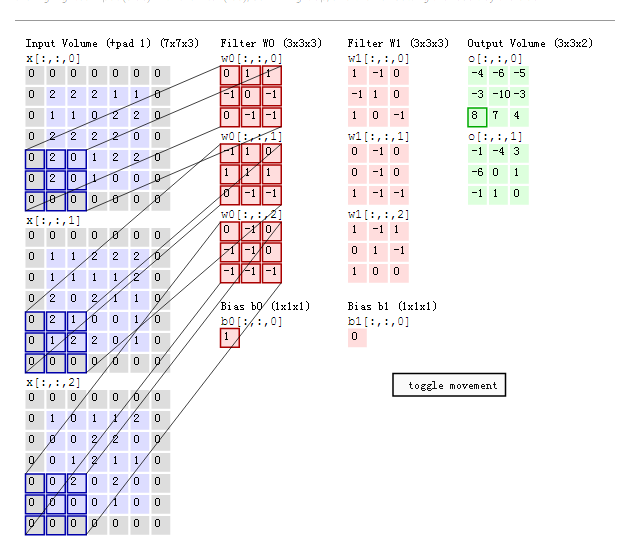
\includegraphics[width=3.0in]{conv.png}
	\caption{卷积操作的示意图}
\end{figure}

除此之外,很多不同形式的卷积更加注重对于图像信息提取的卷积形式也被提出,比如为了减少计算量而增加网络深度的1x1卷积\cite{1x1CONV},为了扩大感受野而获取更多图像信息的放射卷积\cite{DILUTECONV},为了能够对于图片中具体图像有细节感知的形变卷积\cite{DEFORMCONV}等,他们都不再局限于对于固定范围内特征值进行卷积,而是着重于在输入特征图上更多具有影响力的范围内进行输入位置的选取。

\subsubsection{池化层}
池化(Pooling)层可以相比于信号处理中的采样操作,一般对于输入的特征图片图进行降采样操作,从而起到去除噪声,增加网络的平移不变性和旋转不变性,提升整体的训练效果。
事实上池化层有时也被用作上采样,也就是uppooling,通过输入的特征图进行等间隔复制的方式得到原尺度多倍的输出,也就是常见的放大操作。但是随着卷积神经网络的发展至今,人们开始主要使用反卷积的方式来实现上采样的操作,以至于uppooling的操作慢慢不被人所熟知。池化层的超参数包括:
\begin{enumerate}
\item KernelH,KernelW 高宽方向上的池划范围大小 
\item StrideH,StrideW 高宽方向上的池化步长
\end{enumerate}
输入输出参数包括:
\begin{enumerate}
\item Channel,Height,Width 分别为输入通道数、输入高度、输入宽度
\item  Coutput,Houtput,Woutput 分别为输出通道数、输出高度、输出宽度
\end{enumerate}
其中输出参数由如下公式确定:
\begin{equation}[h]
{
\begin{split}
 & Woutput= \frac{Winput-KernelW}{StrideW} +1 \\
 & Houtput= \frac{Hinput-KernelH}{StrideH} +1 \\
 & Coutput= Cinput
\end{split}
}\end{equation}
池化层的计算公式如下:
\begin{equation}[h]
{
x_j=poolmethod(x_i) \qquad  i\in (poolsacale)
}
\end{equation}
pool scale和conv scale类似,是指一次池化操作中对应的$kernel_h*kernel_w$范围
poolmethod 代表 的是具体的下采样函数。
通常有三种类型,一种是最大型池化,在poolscale中选取值最大的数作为结果的输出;一种是均值型池化,将poolscale中的数值求和做平均输出,还有是随机型池化,也就是将poolscale中的数值随机选取进行输出。
其中最大型池化使用最为广泛,因为其最能够体现池化层对于平移和旋转操作的鲁棒性,而均值池化层主要用在特征归一化操作和最后高位信息的整合上面,以最常见的max-pooling操作为例,具体的计算示意图如下:
\begin{figure}[!ht]
 \centering
	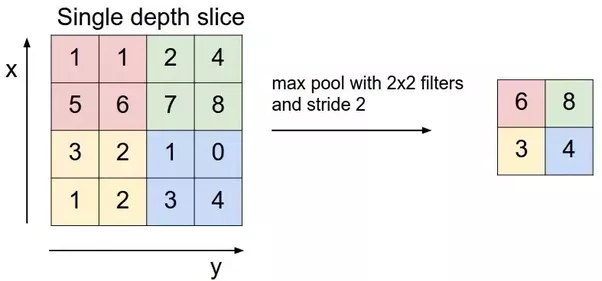
\includegraphics[width=3.0in]{pooling.png}
	\caption{max-pooling的操作示意图}
\end{figure}

和卷积层的发展类似,pooling层也慢慢发展出很多不同的分支,除了前面提到的 up pooling层之外,在物体检测中存在着使用非常广泛的roi-pooling\cite{ROIPOOLING}和空间金字塔pooling(也就是sppnet)\cite{SPPNET}。
\subsubsection{全连接层}
全连接(Fully-connected,FC)层
是普通机器学习方法中使用最多的层,包括SVM,随机森林,boosting种处处可见与之呼应的操作,简单来讲输入的类似于一维向量通过一个矩阵做矩阵乘法运算得到另一个一维向量的过程。

全连接层使用过程中需要设定输出大小即可,其自身的参数是一个输入大小乘以输出大小的矩阵,如果采用带有偏置的算法则还需要一个和输出长度相同数目的偏置项,总结来讲全连接层的参数包括:
\begin{enumerate}
\item $Fc_input$  输入大小
\item $Fc_output$ 输出大小
\item $Fc_W$ 		  模型参数W
\item $Fc_b$ 		  模型参数偏置项
\end{enumerate}

具体的计算过程可以通过公式进行表达:
\begin{equation}{
Fc_j=X_i·W_j^T+bj
}
\end{equation}
从实现的角度上看,可以比较明显的看出全连接层的整体实现可以通过矩阵乘法来完成,通过和卷积层类似的方法将所有的特征输入扩展成多维的等长向量也就是矩阵然后通过,矩阵乘法来快速的将全连接层的相关问题进行实现。如下是输入为800,输出为500的全连接层示意图。
\begin{figure}[!ht]
 \centering
	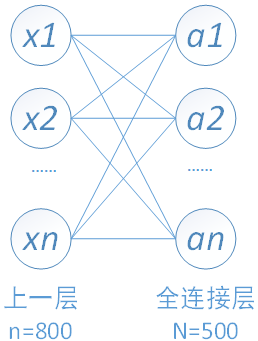
\includegraphics[width=1.50in]{inner.png}
	\caption{全连接层的操作示意图}
\end{figure}

但是需要注意的是,在使用过程中,全连接层的的参数量是$n^2$也就是说全链接层很容易出现参数量过大的问题。比较著名的案例就是VGGnet\cite{VGGNET}中最后的三个FC层,几乎占据了整个网络一半的参数量,
实际中完全可以使用1x1卷积\cite{1x1CONV},global pooling\cite{1x1CONV}等类似的操作对其进行替代以减少参数量。
但是在最新的研究中发现,全链接层可在模型表示能力迁移过程中充当“防火墙”的作用。具体来讲,假设在一个数据库中上预训练得到的模型为 ,则该数据库可视为源域(迁移学习中的source domain)。微调(finetuning)是深度学习领域最常用的迁移学习技术。针对微调,若目标域(targetdomain)中的图像与源域中图像差异巨大(如相比ImageNet,目标域图像不是物体为中心的图像,而是风景照),不含FC的网络微调后的结果要差于含FC的网络。因此FC可视作模型表示能力的“防火墙”,特别是在源域与目标域差异较大的情况下,FC可保持较大的模型capacity从而保证模型表示能力的迁移。也就是说,冗余的参数并不一无是处\cite{FCGOOD}。
\subsubsection{归一化层}
归一化层指的是对每一层的输出进行标准化操作,使得下一层的输入保持一个 较为稳定的分布。常用的标准化层有局部区域归一化(Local Region Normalization, LRN)层,批量标准化(BatchNomalization,BN)\cite{BN}层等。这里着重介绍一下BatchNormalization层:

BatchNormalization也就是批量规范化,在网络训练时,对每个minibatch的特征在卷积之后做一次规范化,使得其输出的特征为零均值和1方差的,在加入两个动态学的参数,尺度(scale)和偏移(bias),用于还原最初的输入,从而保证整个网络的表征能力。实际上,BN层的引入本质上是为了使得每一个卷积层的输入数据的分布统一化,即保证相同均值与方差。另外一个主要的原因则足防止梯度消失,通过将输入归一化到固定的均俏和方差,使得原本尺度很小的特征相应变火,后馈计算时其梯度也相应增大,从而很好的防止梯度弥散。

BN层的参数包括global status(使用网络参数中的均值方差还是根据输入数据重新计算)、moving average fraction(每次计算的累加方式)、eps(为了防止方差为了0加入的偏置项)
\begin{figure}[!ht]
 \centering
	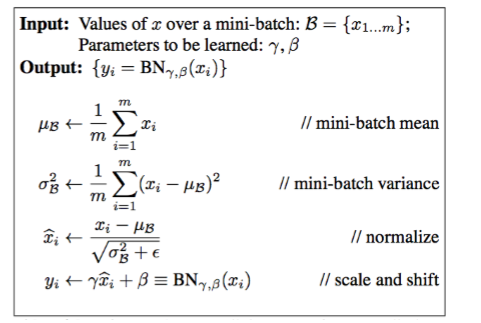
\includegraphics[width=3.0in]{BN.png}
	\caption{BN层的操作说明}
\end{figure}

BN的提出在神经网络的发展过程中具有非常重要的意义,大大改善了神经网络的收敛问题,也可以说从某种程度上改进了神经网络的整体效果。
\subsubsection{损失函数loss层}
Lossfunction是神经网络中用来衡量网络预测和真实值之间的误差情况,最常用的决策层损失函数是:Softmax损失函数和欧几里得损失函数。

Softmax 损失函数主要用于多分类任务,其具体的损失函数表达为:
\begin{equation}{
l(y,z)=-log\left (  \frac{e^z_y}{\sum_{j=1}^{m} e^z_j} \right )
}
\end{equation}
其中m表示分类的类别总的数目,y表示标签,z表示网络预测的类别。也就是说将所有类别的预测值取他们的指数值求和,然后判断实际标签中样本在其中所占的比重,并将其取log作为loss函数和优化的值。

欧几里得损失函数主要用于回归任务,具体的回归损失函数如下:
\begin{equation}{
l(y,z)=(z-y)^2
}
\end{equation}
其中y,z同softmaxloss的含义相同。

除了这两种常用的loss函数之外,还有比如交叉熵损失函数,smooth L1\cite{FASTERRCNN}损失函数等,都是在分类和检测中经常使用的损失函数。

\subsection{卷积神经网络常用激活函数}
卷积输出之后通常会使用激活函数进行非线性激活,从而增强网络的模拟变换能力,不然只是线性变化的组合可以涵盖的空间非常有限.下图总结了神经网络中经常使用的激活函数:
\begin{figure}[!ht]
 \centering
	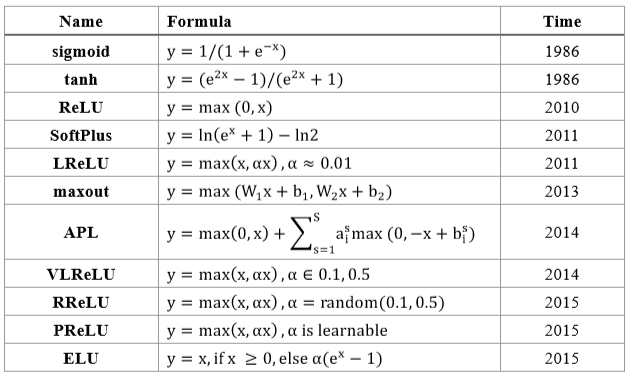
\includegraphics[width=4.0in]{nolinearfunc.png}
	\caption{激活函数的具体表达式以及出现时间}
\end{figure}

其中比较重要的是sigmoid函数、relu函数、以及prelu函数,下面是他们的函数曲线图:
\begin{figure}[!ht]
 \centering
	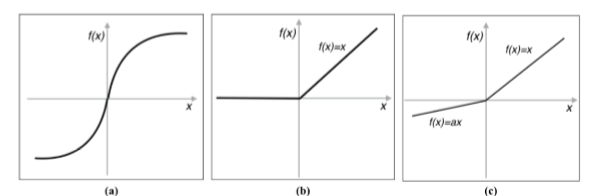
\includegraphics[width=4.0in]{reluprelu.png}
	\caption{sigmoid(a)、relu(b)、prelu(c)函数的函数曲线示意图}
\end{figure}

\subsubsection{sigmoid函数}
sigmoid函数是神经网络最早使用的激活函数,从函数的特性上可以看到其能把输出映射到区间 (0,1):若输入趋于负无穷,则趋近于 0;若输入趋于正无穷,则输出趋近于 1。
近年来由于梯度下降法的使用增加,sigmoid在数值较大的情况下,导数趋近于0,这样导致的后果则是对应的梯度也会慢慢消失,导致训练的过程变得缓慢难以得到正常的收敛效果。
\subsubsection{relu函数}
RELU(Rectified Linear Unit)激活函数,中文也称修正式线性激活函数。由于自身的非饱和特性,修正式线性单元极大 程度的加速了深度卷积网络的收敛。但是修正式线性单元也存在一个很大的问题。 在训练的时候,修正式线性单元比较脆弱并且可能“死亡”。举个例子来说,当一个 很大的梯度流过修正式线性单元的神经元的时候,可能会导致梯度更新到一种特别 的状态,在这种状态下神经元将无法被其他任何数据点再次激活。如果这种情况发 生,那么从此所以流过这个神经元的梯度将都变成 0。也就是说,这个单元在训练中 将不可逆转的死亡,而这样会导致数据多样化的丢失。
\subsubsection{prelu函数}
prelu函数在负轴上加入了固定大小斜率的$a$,从而确保梯度不会因为突然死亡的问题而导致网络崩溃。

除此之外,tanh是作为sigmoid函数在(-1,1)域上的扩展,
ELU函数是RELU和prelu函数在负值域上的变换斜率的优化方式。MAXOUT是是使用更加粗暴的阶段方式对于神经网络进行截取来获得非线性的激活函数。
\subsection{卷积神经网络常用的参数初始化方法}
神经网络求解的是局部最小值,一个好的参数初始化方法能使得卷积神经网络 收敛且收敛的更快。常用的卷积神经网络初始化方法有如下几种。
\begin{enumerate}
\item 常数初始化:使用固定的常数初始化每个参数,常用来初始化的常数一般比较小,通常为 0。 常数初始化方法通常对偏置项所使用。
\item 均匀分布初始化:假设参数服从在区间 [l,h] 上的均匀分布,进而为参数进行初始化。通常为权重 参数使用。

均匀初始化方法中比较常见的是在 2010 年提出的Xavier\cite{XAVIER}方法 ,Xavier 初始化方法Xavier 初始化方法能够使得每 一层的输出方差尽量相等,从而让网络中的信息更好的流动。具体表达式为:
\begin{equation}{
W=U\left [ -\sqrt{\frac{6}{n_{input}+n_{output}}}, \sqrt{\frac{6}{n_{input}+n_{output}}} \right ]
}
\end{equation}

\item 高斯分布初始化:为0方差的高斯分布,$\sigma$为参数进行初始化。通常为权重参数使用。$\sigma$可以是人为制定也可以是通过输入输出计算得到。

比较流行的高斯分布初始化的方法是MSRA\cite{MSRA},由微软亚研院提出,具体公式如下:
\begin{equation}{
W \sim N\left [ 0, \sqrt{\frac{4}{n_{input}+n_{output}}}\right ]
}
\end{equation}
实验证明,对于较深的 卷积神经网络,MSRA 初始化方法比 Xavier 初始化方法更容易收敛。
\item gabor初始化\cite{GABOR}:gabor初始化的方法是根据gabar filter的参数直接作为神经网路的参数,一般在网络的第一层进行使用。由于其具有天然的图像滤波特性,所以很多时候可以固定参数。不对其就行学习,从而达到减轻训练时间和负担的作用,从下图中可以看到针对于不同的模式识别任务使用gabor滤波器都可以降低 31-35%的能耗。
\end{enumerate}
\begin{figure}
includegraphics[width=4.0in]{gaborenergy.png}
\caption{使用gabor固定初始化训练对于消耗能源的降低}
\end{figure}

\subsection{卷积神经网络的训练与优化}
 通常对于包含N个数据的数据集D ,优化的损失函数可以写成:
\begin{equation}{
J(W,b)=\frac{1}{N}\sum_{i=1}^{N}l(y_i,z)+\lambda \Phi (W)
}
\end{equation}


以具有动量的SGD梯度下降方法为例:
\begin{equation}
\begin{split}
&V_{t+1}=\mu V_t-\alpha \bigtriangledown l(W_t) \\
&W_{t+1}=W_t+V_{t+1}
\end{split}
\end{equation}
其中 t+1 是迭代的当前轮数,W 是需要更新的参数, $a \bigtriangledown l(W_t)$是目标损失函数对于 $W_t$的偏导数,$V_t$ 是上一次参数的更新量,$V_{t+1}$ 是本次的参数更新量, $\mu$ 是动量值, $\alpha$ 是学习率。

卷积神经网络的训练主要使用基于梯度的反向传播(Backpropagation,BP)算法。 假设卷积神经网络一共有 N 层,记作 $L_1\cdots L_n$,y代表样本标签,z 代表每一层的输出,a代表每一层输出的激活值,$\delta$代表每一层传回的梯度值,$W$为权重,$b$为偏置项,则BP算法步骤如下:
\begin{enumerate}
\item 进行前馈运算,利用前向传导公式,得到 $L_1\cdots L_n$的激活值
\item 对 LN 层,计算损失函数对应的偏导值
\item 对于第 i 层 Li,i = N−1,...,2,计算输出的梯度
\item 依次计算每一层参数的梯度
\item 利用更新的公式更新参数值。
\end{enumerate}

\section{神经网络训练速度的提升}
在大型数据集上进行训练的现代神经网络架构可以跨广泛的多种领域获取可观的结果,领域涵盖从语音和图像认知、自然语言处理、到业界关注的诸如欺诈检测和推荐系统这样的应用等各个方面。但是训练这些神经网络模型在计算上有严格要求。尽管近些年来 GPU\cite{CUDA} 硬件、网络架构和训练方法上均取得了重大的进步,但事实是在单一机器上,网络训练所需要的时间仍然长得不切实际。幸运的是,我们不仅限于单个机器:大量工作和研究已经使有效的神经网络分布式训练成为了可能。多机多卡训练也可以理解为分布式训练,但是由于传统的分布式训练主要基于cpu进行计算。而现代深度学习的分布式框架学习,gpu的使用是其中不得不实现的一个部分,所以多机多卡的形容更加贴切。

关于多机多卡的训练策略和普通的单机训练相面临更多的挑战,作为研究生生涯中非常感兴趣的一部分,也是整个神经网络实验的基础研究部分,将我对于多机多卡的一些调研和感悟简单做介绍:
\subsection{并行模式}
多机多卡训练一般有两种模式:数据并行和模型并行。

模型并行(model parallelism),在分布式系统中的不同机器分别负责在单个网络的不同部分计算——例如每层神经网络可能会被分配到不同的机器。

数据并行(DataParallelism),不同的机器有着整个模型的完全拷贝;每个机器只获得整个数据的不同部分。计算的结果通过某些方法结合起来。
\begin{figure}[!ht]
 \centering
	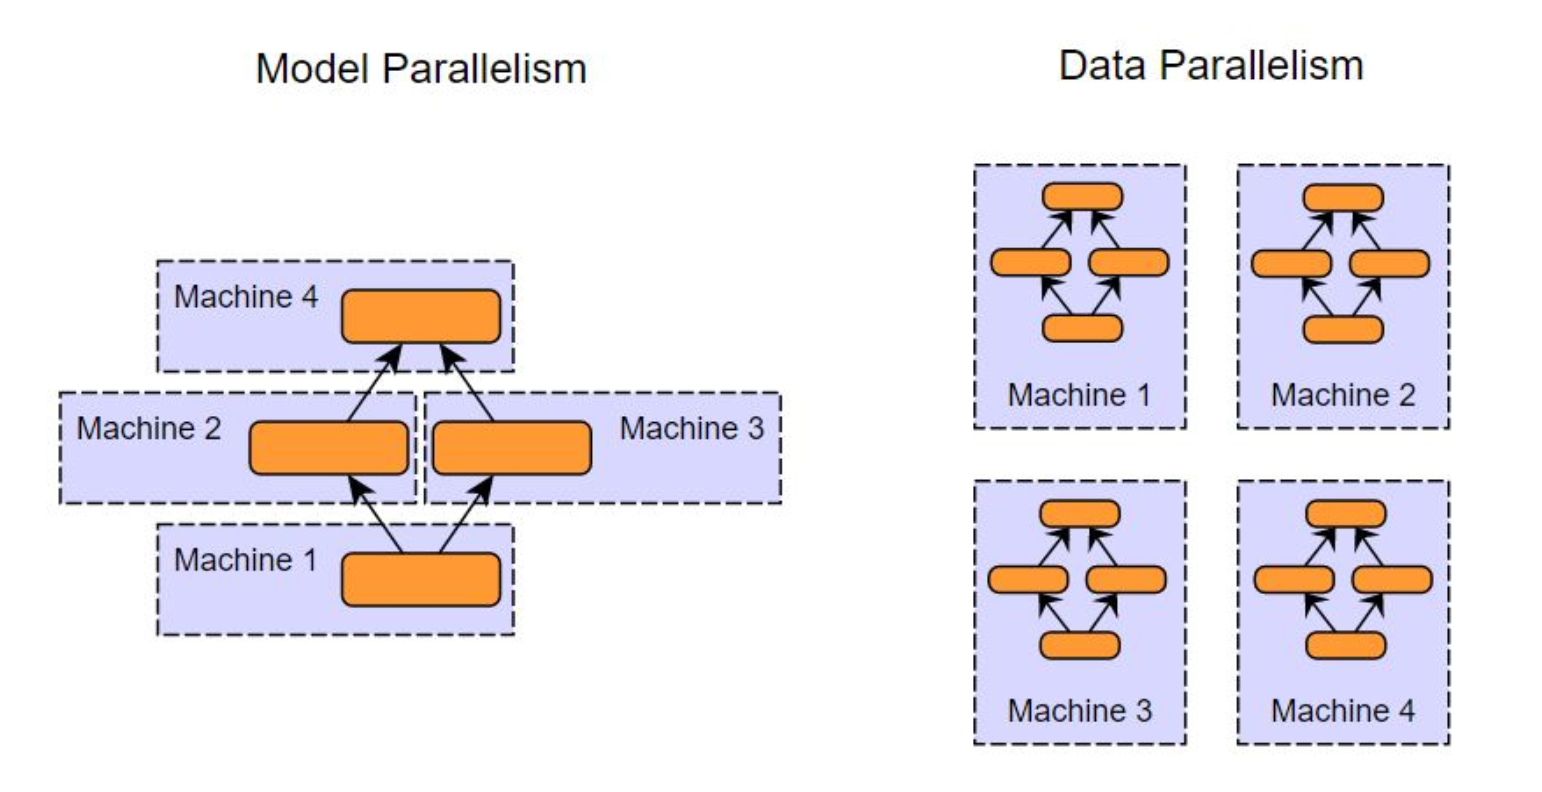
\includegraphics[width=5.0in]{modeldatapara.png}
	\caption{模型并行与数据并行示意图}
\end{figure}

当然,这些方法并不是互相排斥的。想象一个多GPU 系统的集群,我们可以对每个机器使用模型并行(将模型分拆到各个 GPU 中),并在机器间进行数据并行。
尽管在实践中模型并行可以取得良好的效果,但数据并行毫无争议是分布式系统中最适的方法,而且也一直是更多研究的焦点。实现性、容错性和好的集群利用率让数据并行比模型并行更加简单。分布式训练中的数据并行方法在每一个 worker machine 上都有一套完整的模型,但分别对训练数据集的不同子集进行处理。数据并行训练方法均需要一些整合结果和在各工作器(worker)间同步模型参数的方法。

\subsection{参数更新方式}
对应着数据并行训练方式,如何对于参数进行更新也就成了非常关键的问题,目前比较主流的参数更新方法有两种:参数平均化的更新方式,异步随机梯度下降的方式。

\textbf{参数平均化:}参数平均化是概念上最为简单的数据并行方法。使用参数平均时,训练按照如下方式执行:
\begin{enumerate}
\item 根据模型配置随机初始化网络参数
\item 将现有的参数的一个副本分配给每一个 worker machine
\item 在该数据的一个子集上对每一个 worker 进行训练
\item 从每一个 worker 的平均参数上设立一个全局参数
\item 当还需要处理更多数据时,回到第 2 步
\end{enumerate}

同参数平均化相似的方法是:基于更新的数据并行化(update based data parallelism)。
两者的基本区别在于:不会将参数从 worker 传递给参数服务器,而是传递更新
(例如:梯度柱型的学习率和动量(gradients post learning rate and momentum))当我们放松同步更新的要求时,
基于更新的数据并行变得越来越有趣(毫无疑问它更有用)。即在更新参数的变化值被计算的时候就应用于参数向量(而不是等待所有 worker 的 N ≥ 1 次迭1代)。这就催生了异步随机梯度下降算法

\textbf{异步随机梯度下降:}
异步的随机梯度下降故顾名思义,根据一定的算法对于多个machine的更新的过程进行权衡处理,但是保持训练机器的训练过程不中断,可以预见异步随机梯度下降有两个主要优点:
首先,潜在可能在整个分布式系统中获得更高的通量:worker 可以将更多时间花在执行有用的计算而不是等待参数平均化步骤完成。
其次,worker 有可能可以集成来自其它 worker 的信息(参数更新),这比使用同步(每 N 个步骤)更新更快
通过在参数向量中引入异步更新,也引入了一个新问题,也就是过期梯度问题(stale gradient problem)。
过期梯度问题的产生是因为梯度(更新)的计算需要时间,在一个 worker完成这些计算并将结果应用于全局参数向量前,这些参数可能已经更新过许多次了,所以如何设定这些更新的策略也是现在多机多卡的研究热点所在。

\subsection{基于机器学习框架的多机多卡训练}
\subsubsection{caffe中的多机多卡}
caffe\cite{CAFFE}是由贾扬清开发的轻量级C++深度学习框架,因为其出现时间早,计算速度快等优势被Alex用于训练imagenet并且大获成功,从而大获成功,是影响比较大的学习框架之一。
作为用户,在caffe中实现多卡训练比较简单,主需要在命令行中设置参数 -gpu  gpu\_ID 就可以选择希望占用的GPU。在综合了代码和测试效果来看,caffe是采用了数据并行,参数平均化更新的策略,实际测试中也可以很明显的看到默认0卡的显存占用更大,而且存在一定的间隔内,显卡中的使用率是会有明显空缺的,除去数据读取的原因之外,参数同步也是其中重要的一部分原因。

在nVidia开源的nVidia-caffe中,则大胆的采用了异步的SGD参数更新方式,可以很明显看到不仅训练的速度快,而且由于其训练和测试都被分摊到了单独的显卡,而不是都在0卡上进行同步,导致其训练的所占用的显存要比普通的caffe版本更加小很多,但是所带来的问题也同样明显,在训练的过程中可以明显看出其收敛的稳定性不够出色,同样的训练参数和训练数据在普通的caffe中训练,可以收敛loss曲线也非常平稳,但是nVidia-caffe中却迟迟不能收敛,而且网络的训练也不够稳定,易出现崩坏的情况。

再来看基于分布式的多机多卡训练,在intel/caffe中提供了多机多卡的训练方式,使用的方式稍微复杂,需要安装ansible,然后在用来训练的机器上配置好主机的SSH公钥验证,然后使用ansible统一安装caffe所需要的软件同时编译caffe,设置好同步的文件夹,然后就可以选择需要的训练配置文件和数据就可以了。使用mpi 命令配合执行caffe train命令就可以实现多机分布式训练网络。

综合来看,从工程上来讲,目前的分布式的多机训练其实是建立以往分布式训练的基础之上,有很强的spark和Hadoop烙印,对于多卡训练,大多数的实现都是基于nvidia-NCCL(Nvidia Collective multi-GPU Communication Library)的多GPU通信库。NCCL是Nvidia Collective multi-GPU Communication Library的简称,它是一个实现多GPU的collective communication通信(all-gather, reduce, broadcast)库,Nvidia做了很多优化,以在PCIe、Nvlink、InfiniBand上实现较高的通信速度。

而从算法上来看,无论是同步训练还是异步训练其实都有其各自的挑战,对于同步训练来讲,虽然一定程度上加速了网络的训练速度,但神经网络在batch数目较大情况下的优化其实不是一帆风顺,而且随着cluster的数目增加,同步时延会成为性能关键,树形和环形拓扑都会成为其下一步的改进方向。

实际上异步算法更加受到人们的期待,就是因为其一定程度上摆脱了同步时延限制,能够实现了硬件性能的线性加速。从其他机器学习的时间和发展过程来说,如果深度学习的使用得到广泛的应用,那么异步算法的优化就会是大势所趋,因为对于实际应用的成本压缩和人们的对于性能的追求决定了算法的方向。

\section{神经网络前馈速度优化}
网络前馈又被称为网络的inference,一般是指经过一定的数据训练,对于输入数据和输出结果具有一定正向的科学计算过程,可能这样的说法不是很准确,因为很多时候为了获得更为理想的判断结果,往往会采取人工检查和机器过滤的两种方式进行结合,那么在我的工作之中主要是对于机器过滤中对于所需要使用的科学计算过程所进行的一些速度上的优化。具体算法的表述形式可以参照2.1节中的神经网络的基础算法过程进行对比。
\subsection{卷积计算的优化方式}
对于卷积层的优化有三个方向,第一种是对于目前的算法下,通过编程技巧减少内存瓶颈和增加缓存命中率的方式直接对卷积的过程进行优化;第二种相对比较直接,是直接使用包装成熟的第三方的加速库如blas,FFT等对卷积计算进行加速,而实际上这些库使用的加速方法和第一步是类似的,但因为类似的加速库都会从汇编级指令进行不必要操作的剪除所以效率上会有很大的改进;第三种是结合数据结构和矩阵理论的算法对于卷积的操作进行创新和改良。在这三个方向中,第一种适合大部分操作系统平台Windows/Mac/Linux/Unix/Arch等,和CPU计算平台,如intel/AMD/ARM/PpwerPC/龙芯等,相对来说扩展性和移植性都非常的出色,适合具有一定开发能力的团队核心开发和使用。第二种方法主要会依赖于计算库的特性,具有一定的适用范围,包括操作系统和CPU环境等。第三种方法则一般局限于理论研究,通过以减少算法复杂度的方式来减少卷积的计算量,也是理想情况下加速卷积速度的最佳选择,但在实际计算机内存和缓存架构上并不一定的可以取得良好的效果。
\subsubsection{通过编程优化卷积速度}
CPU直接计算卷积:正如之前的基础知识中介绍的,普通的卷积操作需要对于输入特征中的 N,C,H,W四维数据中进行提取,然后和卷积参数中Coutput,Cinput,kernelH,KernelW各个维数中的参数进行分别点乘,通常的写法使用for循环进行完成的话,需要使用7个for循环来完成:
\begin{figure}
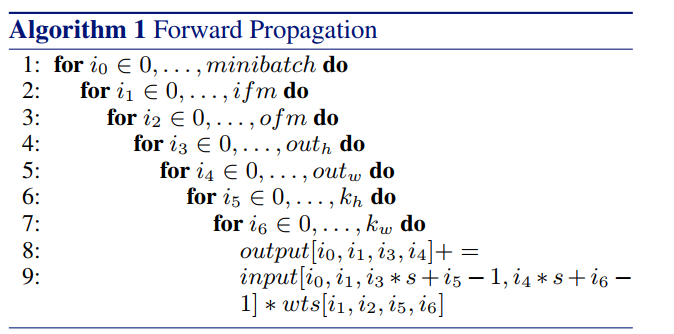
\includegraphics[height=3.0in]{CONVFOR.png}
\caption{使用7层FOR循环实现卷积操作}
\end{figure}
这种粗暴的实现方式会使用N*Cinput*Coutput*Woutput*Houtput*KernelW*kernelH次乘法和加法操作,并且读取相同次数的内存。所以有很多优化的可能性。

首先通过选择合适的特征图存取方式减少内存读取费用:普通的特征图计算,按照图片个数、通道数、特征图长、特征图宽的顺序存储;但是在实际读取过程中,对于通道数这一层是读取负载最重的,应该将不同通道之间的读取负载降低。于是内存存储上使用普通的特征图计算,按照图片个数、特征图长、特征图宽、通道数的顺序存储会更加合理。

其次通过使用SIMD指令集和并行向量处理机的提高计算速度:
向量处理器,又称数组处理器,是一种实现了直接操作一维数组(向量)指令集的中央处理器(CPU)。并行向量处理机一个最大的优点是它能够允许软件传递大量的并行任务给硬件。

向量处理机所配合使用的指令集主要是指SIMD(Single Instruction Multiple Data)顾名思义就是“一条指令处理多个数据(一般是以2为底的指数数量)”的并行处理技术,相比于“一条指令处理几个数据”,运算速度将会大大提高。而只需要一条很短的指令即可。在SSE4指令集中可以一次进行4次乘法操作,而在AVX512指令集中,可以一次完成16个float的乘法。结合这一思想,可以有效加速对于卷积中的乘法操作。尤其在移动端的优化计算种,
\subsubsection{卷积的快速算法}
im2col+GEMM\cite{CAFFE}:imcol+gemm最常见的卷积快速算法是imcol+gemm,(gemm是矩阵乘法的简称),在卷积层的介绍中,可以看出笔者把卷积的每一个输出值都用多个输入数据和卷积层参数值相称的求和的方式表示,也就是向量积,一共需要做Coutput*Houtput*Woutput次这样的向量乘法,而且每次向量乘法的维数都一致,所以可以通过矩阵乘法来实现相关操作,具体的操作可以参见下图
\begin{figure}[!ht]
 \centering
	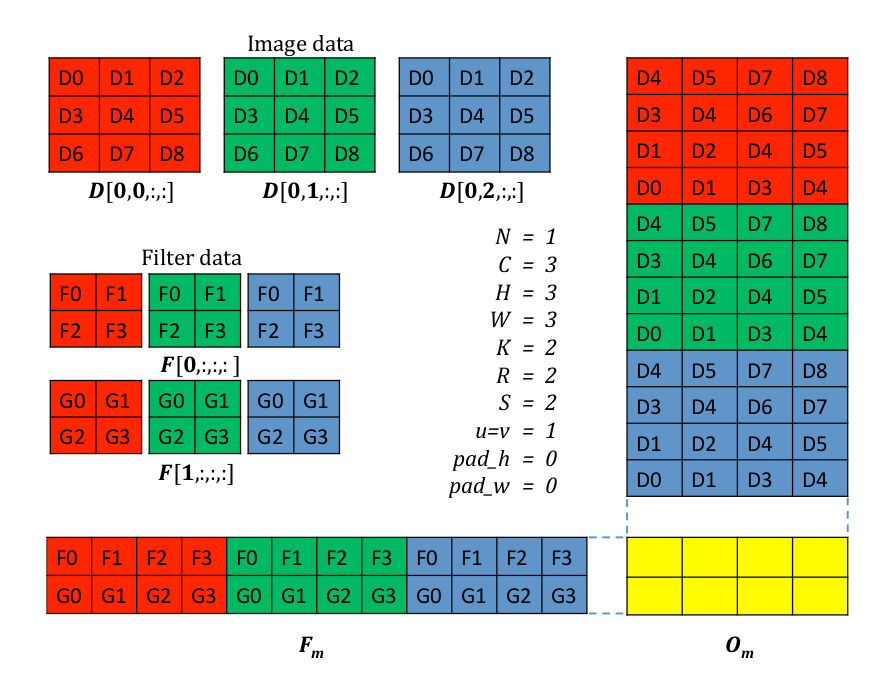
\includegraphics[width=4.0in]{im2col.png}
	\caption{im2col的操作示意图}
\end{figure}

Winograd卷积算法\cite{WINOGRAD}:得益于Shmuel Winograd之前对于计算机超算的工作,可以使用线性代数分解的方式将一些固定卷积核尺寸大小卷积操作如2x2,3x3等,分解成多个具有固定参数的小矩阵相乘的方式,从而大幅度提升了卷积的速度。
\begin{figure}[!ht]
 \centering
	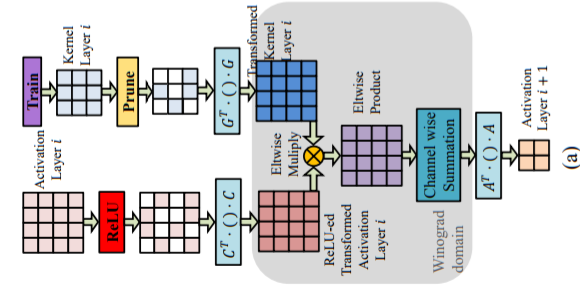
\includegraphics[width=4.0in]{winograd.png}
	\caption{winograd算法的算法过程}
\end{figure}

MEC\cite{MEC}:im2col+gemm的改进版,在减少内存的同时顺便可以提升一些速度。
\begin{figure}[!ht]
 \centering
	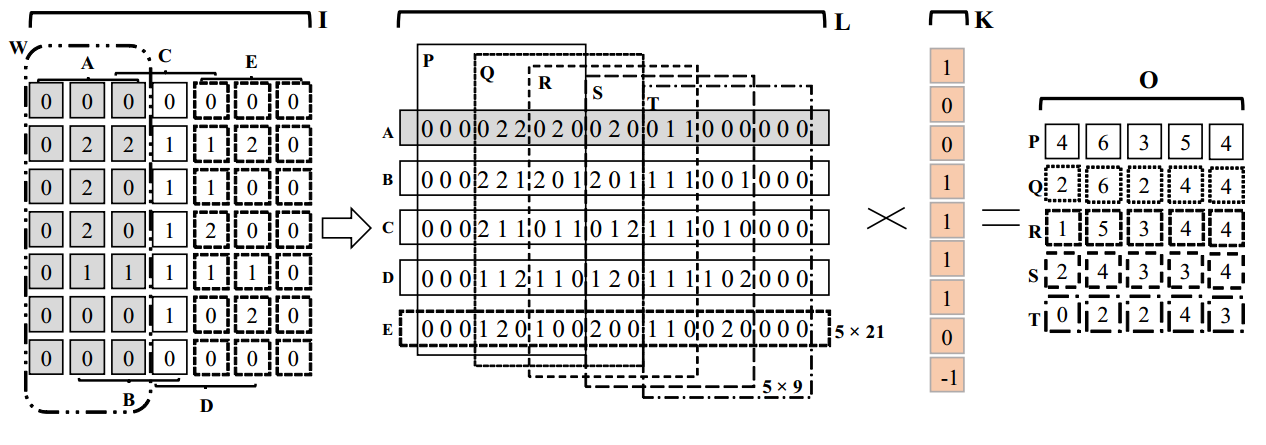
\includegraphics[width=4.0in]{MEC.png}
	\caption{MEC算法的算法过程}
\end{figure}

\subsubsection{借助第三方的计算库对于卷积计算进行优化}
\begin{enumerate}
\item 
在使用im2col+GEMM的过程中,矩阵乘法的计算是主要的计算过程,而在世纪的工程开发过程当中,矩阵乘法可以借助openblas、MKL、altblas等的线性代数优化库,可以有效地提升时间。
\item 使用MKL和MKLDNN\cite{MKL}中的卷积层实现,用于深度神经网络的英特尔数学内核库(MKLDNN)是用于加速intel体系结构上的深度学习框架的深度学习应用程序的开源性能库。intel MKL-DNN包括高度矢量化和线程化构建模块,用于实现具有C和C ++接口的卷积神经网络(CNN)。
\begin{figure}[!ht]
 \centering
	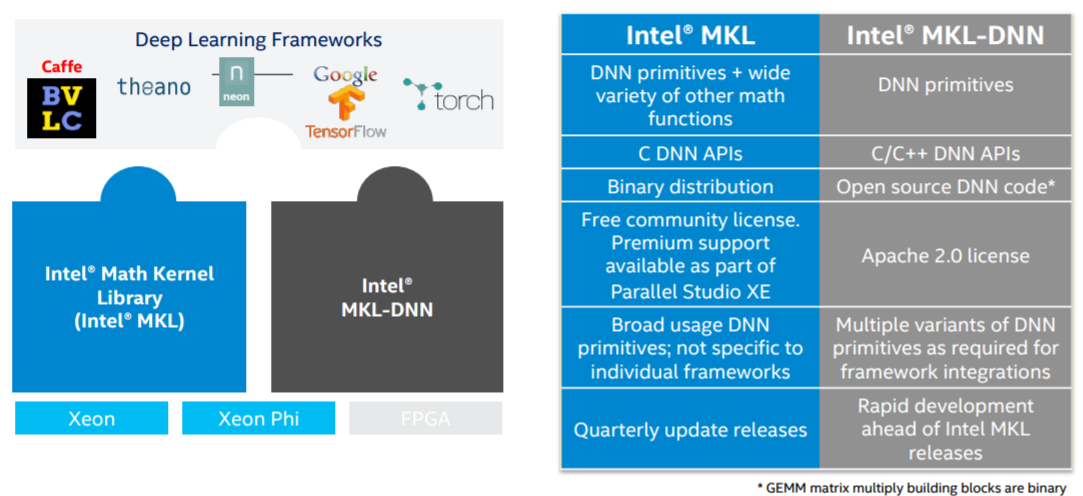
\includegraphics[width=4.0in]{MKLLOGO.png}
	\caption{MKL/MKL-DNN的简介}
\end{figure}
\item 使用NNPACK\cite{NNPACK}中的FFT卷积操作,NNPACK也是神经网络计算的加速包,基于傅立叶变换和Winograd变换的快速卷积算法,优势在于没有附加的依赖库,非常适合于移动端的开发。
\begin{figure}[!ht]
 \centering
	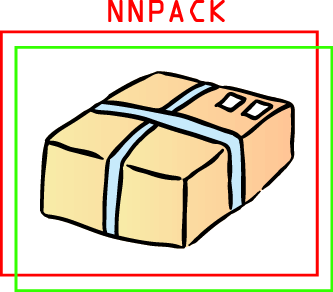
\includegraphics[width=2.0in]{nnpack.png}
	\caption{nnpack}
\end{figure}

\item 使用CUDNN\cite{CUDNN}和TensorRT中的卷积实现,cudnn和tenorRT是使用在gpu上的算法加速库,都是nVidia为了加速神经网络而开发的闭源库,但是可以通过下载现有的公开库进行使用,cudnn和tensorrt是所有加速库中能够获得加速比最高选择,原因在于其对于GPU的出色使用。
\begin{figure}[!ht]
 \centering
	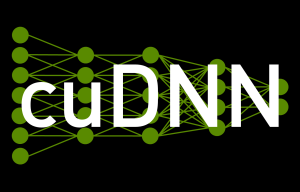
\includegraphics[width=2.50in]{cudnnlogo.png}
	\caption{CUDNN}
\end{figure}
\end{enumerate}

\subsection{不同网络层的合并}
事实上,随着神经网络的不断发展,卷积神经网络的层的种类其实是不断扩充的,有很多在随后的岁月中被发明并且广泛的使用,如BatchNorm层、relu层等等,这些网络层在图像识别的发展过程中都起到了非常关键的作用,也极大加速了网络训练的收敛速度和预测效果,但是在工程的生产实践过程之中,很多网络结构在inference的过程中显得非常冗余,也就是说他们可以和其他的操作进行合并。
\begin{enumerate}
\item scale层和batch norm层的合并,在BN层的介绍之中,在BatchNorm层将输入的特征分布转换均值为0,方差为1的同分布之后,还需要连接一个scale层,让网络重新学习数据的分布,这在训练的过程中,确实确实很有效,但是在前馈的过程中,可以把scale层的参数和batchNorm中的除方差一步结合起来,从而减少计算量和多余的内存使用。
\item BN层和卷积层的合并,接着上面的优化方向,既然scale层可以和BatchNorm层,相互合并,那么同样的道理,我们将batchnorm层中储存的方差的值和卷集中的weights的值相互合并,将batchNorm中的bias除以scale之后和卷积中的bias相互合并,就完全可以在卷积层一层的实现过程中完成所有的计算,而不用再次使用batchnorm层。
\item 卷积层和relu层的合并,relu层实质上就是一个符号函数,在卷积完成之后,使用使用一个符号函数就可以避免为relu层重新新建层。
\end{enumerate}

\subsection{本章小结}
本章中我们介绍了卷积识别网络中的基本结构和组成包括卷积层,pooling层、全链接层、激活函数、初始化方式、训练方法等。。
同时也介绍了神经网络的加速训练的方法,即多机多卡的训练方式。
为了能够加速神经网络的在现实环境中的使用,同时介绍了神经网络种常见的加速方法。包括卷积层的快速算法和不同网络层的合并等。

总结来讲,这一章的主要内容是作为卷积神经网络的基础。神经网络中训练和测试中的速度优化是具体识别系统在现实中的应用也是算法发展快速迭代的根本。

在接下了的章节中会有很多细节都使用了本章中的技术。可以从下图中简单了解一下具体不同化方式速度对比。
\begin{figure}[!h]
 \centering
	\includegraphics[width=5.0in]{MKL.png}
	\caption{MKL、MKL2017、MKLDNN、openblas加速方法的具体速度}
\end{figure}






